%%%%%%%%%%%% STONY BROOK
%\documentstyle[prb,preprint,aps]{revtex}
%%%%%%%%%%%%



\documentclass[aps,prb,twocolumn,showpacs,superscriptaddress]{revtex4-1}\begin{tiny}\end{tiny}
%\documentclass[aps,prb,preprint,showpacs,superscriptaddress]{revtex4}

%\usepackage{graphicx} % Include figure files
\usepackage{longtable}
\usepackage{amsfonts}
%\usepackage[dvipdfm]{graphicx}
\usepackage{graphicx}
\usepackage{setspace}
%\usepackage{booktabs}

\begin{document}

\title{Direct Simulation of Thermal Conductivity by Molecular Dynamics}

\author{Philip B. Allen}
\email{philip.allen@stonybrook.edu}
\affiliation{Physics and Astronomy Department, Stony Brook University, Stony Brook, NY 11794-3800, USA}
\author{Yerong Li}
\email{li.yerong@outlook.com}
\affiliation{Physics and Astronomy Department, Stony Brook University, Stony Brook, NY 11794-3800, USA}
\affiliation {Department of Intensive Instruction, Nanjing University, Nanjing 210093, China}
\date{\today}

%\begin{spacing}{2}

\begin{abstract}
Classical molecular dynamics (MD) is often used to simulate thermal conductivity ($\kappa$) by a
``direct method'' where a steady state heat current and corresponding temperature gradient are 
created computationally over a simulation cell of thousands of atoms.  
This paper presents a variation of such algorithms, that gives directly $\kappa(q)$,
the Fourier transform of the non-local $\kappa(x-x^\prime)$ that relates $J(x)$ to $\nabla T(x^\prime)$.
The algorithm is tested on the Lennard-Jones liquid and crystal, and shown to be quite efficient.
Knowledge of $\kappa(q)$
permits a controlled extrapolation to the macroscopic $\kappa$, the $q \rightarrow 0$ limit of
$\kappa(q)$.  The nature of this extrapolation is studied using a Debye spectrum and frequency-dependent
relaxation rate $1/\tau_Q \propto \omega_Q^2$.  The aim of
extrapolation is to reduce the error from the finite length of the simulation cell.
Errors associated with the finite width of the simulation cell are also analyzed using the same Debye spectrum. 
\end{abstract}

%\pacs{29.85.-c, 21.10.-k, 23.20.Lv}
\maketitle

%	\newpage
%	\tableofcontents
%	\newpage	

\section{Introduction}

Molecular dynamics (MD) simulation works for insulators at temperature $T$
high enough that quantum lattice dynamics 
is well approximated by classical Newtonian trajectories.  It has the advantage of
treating interatomic forces beyond harmonic theory without requiring perturbation theory.
For thermal conductivity \cite{Visscher,Schelling} 
$\kappa={\rm Lim}_{q\rightarrow0}\kappa(q)$ of a crystal \cite{Allen}, 
the biggest difficulty is that small $\omega_Q$ modes have long mean free paths $\Lambda_Q$.
This means that the current $J$ at one location $x$ depends on temperature $T$ and
temperature gradient $-\nabla T$ at distant locations $x^\prime$.  The relation between
$J(x)$ and $-\nabla T(x^\prime)$ is the non-local conductivity $\kappa(x-x^\prime)$.  The
long range of $|x-x^\prime|$ means rapid variation of $\kappa(q)$ with $q$ and difficulty
taking the $q\rightarrow 0$ limit.  

Although non-locality of $\kappa$ is certainly implicitly acknowledged, it is rarely
\cite{Mahan} regarded as a direct topic of study.  The main methods of MD used
for $\kappa$ are the Green-Kubo (GK) and the ``direct method'' (DM),
also known as ``non-equilibrium molecular dynamics'' (NEMD). 
These are compared, for example, in Ref.\onlinecite{Schelling}.  The former 
computes $\kappa$ {\it via} equilibrium fluctuations averaged over a large supercell with periodic boundaries.
The latter involves external heat which drives the system from equilibrium.  The unit cell
is elongated in the direction of heat flow, and periodic in the perpendicular directions.
Equal heat input and output allows a steady state.  Heating and cooling 
are isolated in separate regions, and ``bulk'' conduction occurs in between,
if the separation is large enough. 

Here we argue that a direct study of $\kappa(q)$ is both warranted and useful
for finding the bulk $\kappa={\rm Lim}_{q\rightarrow0}\kappa(q)$ by NEMD.
The Peierls-Boltzmann equation (PBE) is well adapted \cite{Allen} for study of $\kappa(q)$.
This paper does four things.  First, a particular version of the standard DM is analyzed, where
the long direction of heat flow is also treated with periodic
boundaries (with length $L$, and discrete slabs perpendicular.)
Heat is added in one slab, and removed at an equal rate from
another slab a distance $L/2$ away, fixing the steady state heat current $J$.  
The thermal conductivity $\kappa_{\rm eff}(L)$ is the of ratio of $J$ to the temperature
gradient $-\nabla T({\rm mid})$ at the mid-point.  A rigorous, but complicated, relation between
 $\kappa_{\rm eff}(L)$ and $\kappa(q)$ is worked out.
Second, a method is developed for direct MD simulation
of $\kappa(q)$, by applying and extracting heat in a sinusoidal pattern.  This allows a 
better-controlled approach to the bulk limit.  The present method, proposed 
previously in Ref.\onlinecite{Allen}, uses continuous heating in a sinusoidal pattern.  We
argue that this method also has numerical advantages over more
traditional simulation protocols.  Third, convergence of $\kappa(q)$ towards $\kappa$
is studied by ``direct method'' simulation
for the Lennard-Jones (LJ) liquid and crystal.  Fourth, $\kappa(q)$ is studied 
by the PBE, using a Debye approximation ($\omega_Q=v|\vec{Q}|$
and $1/\tau_Q = (1/\tau_D) (\omega_Q/\omega_D)^2$).  This is used to analyze convergence
as a function of MD simulation-cell size.

\section{Preliminaries}

This paper assumes a simulation cell with periodic boundary conditions.  The atom at
$\vec{r}$ and the atom at $\vec{r}+\vec{R}$ are equivalent, and have the same dynamics.  For simplicity, the 
primitive translation vectors $\vec{R}$ of the simulation cell ($\vec{A}_1, \   \vec{A}_2, \  \vec{A}_3$), are
assumed orthogonal.  For example, in the sample calculations presented later, they are taken
to be $N_1 a \hat{x}, \ N_2 a \hat{y}, \ N_3 a \hat{z}$, where $a$
is the lattice constant, the edge-length of the {\it fcc} conventional cube.   A typical cell has size
$(N_1, \ N_2, \ N_3)=(6, \ 6, \ 80)$; with 4 atoms in the conventional cube, this means
11,520 atoms.  Heating is done in slabs perpendicular to the long vector ${\vec A}_3$.
Therefore, current flows parallel to $\vec{A}_3$,
and $L= |\vec{A}_3|=N_3a$ is chosen as large as computation permits, trying to surpass the 
distance $\Lambda$ of non-local thermal memory.

Boundaries create challenging problems.  Nanoscale heat transfer is typically
dominated by thermal boundary (or Kapitza) resistance \cite{Kapres}.
For study of bulk conductivity, the aim is to
reduce the influence of boundaries.  One can argue \cite{Liang} that periodic boundary 
conditions are not the most favorable way to do this.  However, in this paper, the
simplicity for analysis of periodicity overrules other considerations.   

A further simplification follows computational necessity, and discretizes the temperature $T(\vec{r})$
into slab values $T(\ell)$.  The slabs are layered
in the $\vec{A}_3$-direction, and have width $d=n_S a$ where $n_S$ is a small
integer and a factor of $N_3$.   The number of slabs is $N_S = N_3/n_S$.
Let the variable $x$ denote distance along
the $\vec{A}_3$-axis, perpendicular to slabs.  The slab indexed by the integer $\ell$
is located in the interval $x=\ell d \pm d/2$.  The temperature $T(\ell)$ is found from
the average kinetic energy of the atoms in the $\ell$'th slab.  Heat is transferred
externally into the $\ell$'th cell at a volume-average rate $\dot{e}(\ell)$.  In steady state,
this is balanced by an outward flux $[J(\ell+1/2)-J(\ell-1/2)]/d$.  Both current and
temperature gradient are properties of the junction of two adjacent slabs.  Their steady-state
linear relation is $J(\ell+1/2)=-\sum_{\ell^\prime}
\kappa(\ell,\ell^\prime)\nabla T(\ell^\prime+1/2)$, where the sum runs over the $N_S$ slabs.  
This definition is required by linear math.
Periodicity requires $\kappa(\ell,\ell^\prime)=\kappa(\ell+mN_S,\ell^\prime+nN_S)$
and homogeneity (if the medium is in fact homogeneous) requires that $\kappa(\ell,\ell^\prime)=
\kappa(\ell-\ell^\prime)$.  Corresponding ({\it via} a unitary Fourier transformation) to the $N_S$ distinct slabs, 
there are $N_S$ distinct wave-vectors $q=2\pi n_q/N_S d$, indexed by integers
$n_q$ and distributed in a one-dimensional Brillouin zone.  In the homogeneous
case, the relation is $J(q)=-\kappa(q)\nabla T(q)$.  We will use the same symbols
($\nabla T(\ell)$ and $\nabla T(q)$, for example) for both coordinate space and
reciprocal space representations of the functions, needing the coordinate
$\ell$ or $q$ to clarify which representation.  These ideas were introduced in
Ref. \onlinecite{Allen}, where further properties are explained.  

It is not hard to
extend the usual derivation of the Kubo formula (ref. \onlinecite{AllenFeldman}, for example)
to derive a Kubo formula for $\kappa(x,x^\prime)$ or $\kappa(\ell,\ell^\prime)$.  The
classical limit is
%
\begin{equation}
\kappa(\ell,\ell^\prime)=-\frac{1}{k_B T^2}\int_0^\infty dt < J(\ell+1/2,t)J(\ell^\prime+1/2,0)>
\label{eq:Kubo}
\end{equation}
%



  








\section{Discrete Pair Heating}

Here is a simple version of NEMD simulation.
Energy is added only to slab $\ell=0$ at a volume-average rate $\dot{e}$, 
and extracted only from slab $N_S/2$
at the same rate.  Zhou {\it et al.} \cite{Zhou} did a careful
study of $\kappa$ for GaN by this method.  They discuss, but do not completely resolve, the
issue of how the answer scales with system size.  Here we analyze this
version with the use of periodic boundaries ($\ell=\ell+N_S$).  Zhou {\it et al.} used rigid boundaries. 
Heat current $J_x(\ell+1/2)=\pm (d/2)\dot{e} \equiv \pm J$ flows across
slab boundaries, the plus sign for $\ell$ to the right of an input and left of an output slab, and
the minus sign for opposite cases.  Adding periodic boundary conditions 
permits a simple Fourier representation of $J_x$,
%
\begin{eqnarray}
J_x(q)&=&\frac{1}{N_S} \sum_{\ell=0}^{N_S-1} e^{-iqx(\ell+1/2)} J_x(\ell+1/2) \nonumber \\
&=& \frac{J}{N_S}\sum_{\ell=0}^{N_S/2-1} \left[e^{-iqx(\ell+1/2)} - {\rm c.c.} \right] \nonumber \\
&=& \frac{J}{N_S} \left( \frac{1-e^{-iqL/2}}{1-e^{iqd}} \right) e^{-iqd/2} - {\rm c.c.} \nonumber \\
&=& \frac{J}{iN_S} \left[ \frac{1-(-1)^{n_q}}{\sin(qd/2)} \right]
\label{eq:Jdph}
\end{eqnarray}
%
At $q=0$, the expression $[ \ ]$ in the last line 
of Eq.(\ref{eq:Jdph}) is ill-defined; the correct value is 0, as is also true for all $q$'s with even $n_q$.
Now let us analyze the approximate thermal conductivity,
%
\begin{equation}
\kappa_{\rm eff}(L) \equiv -J/\nabla_x T({\rm mid}).
\label{eq:keff}
\end{equation}
%
That is, the thermal conductivity is taken as the ratio of the actual current $J$, controlled by the
heating rate $\dot{e}$, to the temperature gradient $-\nabla_x T({\rm mid})$ found midway between the 
heat input slab ($\ell=0$) and output slab ($\ell=N_S/2$).  This temperature gradient has the Fourier 
representation
%
\begin{eqnarray}
\nabla_x &T& ({\rm mid}) = \sum_q e^{iqN_Sd/4} \nabla_x T(q) \ \ [N_S/4={\rm half \ integer}] \nonumber \\
&=& \sum_q e^{iqN_Sd/4} \cos(qd/2) \nabla_x T(q) \ \ [N_S/4={\rm  integer}].
\label{eq:nabTdph}
\end{eqnarray}
%
In the case $N_S/4 = {\rm integer}$, the slab $\ell=N_S/4$ lies midway between heat input and output,
so the temperature gradient (needed at the slab mid-point) is taken as the average of the left
and right slab boundaries.  This introduces the factor $\cos(qd/2)$ in the second version of Eq.(\ref{eq:nabTdph}).
Finally, we substitute $\nabla_x T(q) = -J_x(q)/\kappa(q)$ in Eq.(\ref{eq:nabTdph}), and use 
Eq.(\ref{eq:Jdph}) for $J_x(q)$.  Then Eq.(\ref{eq:keff}) becomes
%
\begin{eqnarray}
\frac{1}{\kappa_{\rm eff}} &=& \frac{2}{N_S}\sum_q^{n_q={\rm odd}} \frac{\sin(qL/4)}{\sin(qd/2)} 
\left[ \frac{1 \ {\rm or} \ \cos(qd/2)}{\kappa(q)} \right] \nonumber \\
&=& \left[ \frac{4 \ {\rm or} \ 4\cos(\pi/N_S)}{N_S\sin(\pi/N_S)} \right] \frac{1}{\kappa(q_{\rm min})}
+\{|n_q| \ge 3 \ {\rm terms}\}. \nonumber \\
\label{eq:kqeff}
\end{eqnarray}
%
This is a surprisingly complicated relation between the size-dependent value
of $\kappa_{\rm eff}$ and the Fourier representation $\kappa(q)$.   
From Eq.(\ref{eq:kqeff}), the leading term (at small $q_{\rm min}d/2=\pi d/L$)
is $1/\kappa_{\rm eff}=4/\pi\kappa(q_{\rm min})$, with oscillatory
corrections $~\sum_{n=1} (4/\pi) (-1)^n /[(2n+1)\kappa((2n+1)q_{\rm min})]$.  
In the local limit, $\kappa(q)=\kappa$,
Eq.(\ref{eq:kqeff}) converges exactly to $\kappa_{\rm eff}=\kappa$. 
For crystals, where long-range non-local behavior is caused by long-wavelength
phonons, the answer (for finite $N_S$) is a
less accurate approximation to $\kappa$ than $\kappa(q_{\rm min})$.  
This motivates developing an algorithm for the direct study of $\kappa(q)$.


\section{Sinusoidal Heating Algorithm}

The simulation cell, divided into slabs,
is shown schematically in Fig. \ref{fig:slab}.
We want to modify
the heat input profile.  Instead of the two slab version, let the heat input be of the form
${\dot e}(\ell)={\dot e}(q_{\rm min})\cos(q_{\rm min}x(\ell))$.  
The temperature variation then has the form $T(\ell)=T_0+\Delta T \cos(q_{\rm min}x(\ell))$. 
Since slab temperatures $T(\ell)$ at all $N_S$ values of $\ell$ 
are used to compute the Fourier amplitude $\Delta T$, numerical noise 
averages out faster.


Equation 26 of the previous paper \cite{Allen} says, for arbitrary
heating ${\dot e}(\ell)$, heating rate, temperature, and conductivity
in Fourier space are related by (for $q\ne 0$), 
%
\begin{equation}
\Delta T(q)=\frac{{\dot e}(q)d^2}{4\sin^2 (qd/2) \kappa(q)}
\label{eq:nonlocal}
\end{equation}
%
For simple sinusoidal heating, ${\dot e}(q)$ and $\Delta T(q)$ are zero except
at $q=q_{\rm min}$.  Then the conductivity is
%
\begin{equation}
\kappa(q_{\rm min})=\frac{{\dot e}d^2/\Delta T}{4\sin^2(q_{\rm min} d/2)}
\rightarrow \frac{N_S^2{\dot e}d^2}{4\pi^2 \Delta T}
\label{eq:kappa}
\end{equation}
%
This makes sense:  $\Delta T/N_S d$ measures the size of the temperature gradient, 
and ${\dot e}N_S d$, the heat input per unit area, measures the size of the heat current.
%The factor $\sin^2 (q_{\rm min}d/2)$ appears because of the discretization of the coordinate $x$ to 
%the variable $\ell$ that enumerates the slabs.

 
\par
\begin{figure}[top]
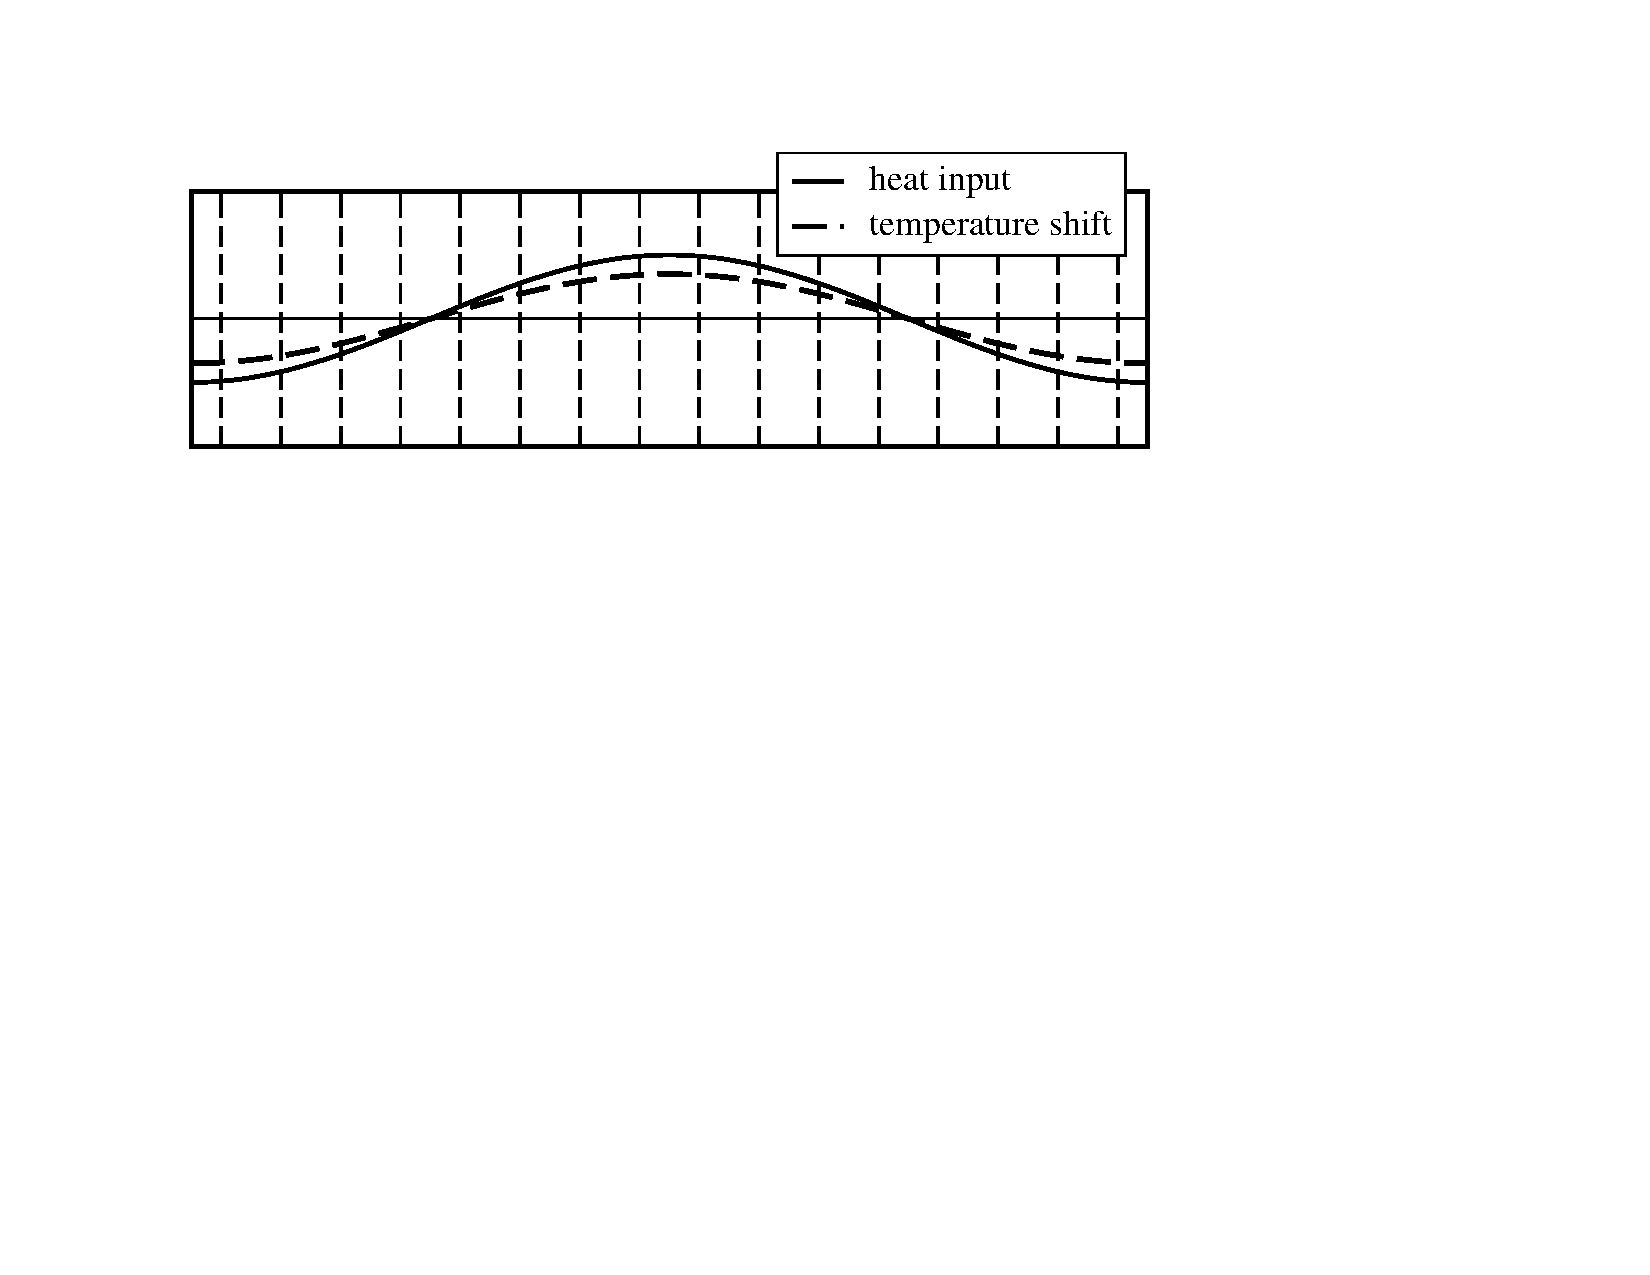
\includegraphics[angle=0,width=0.5\textwidth]{slab.pdf}
\caption{\label{fig:slab} Schematic picture of an $N_S=16$ slab simulation cell
with periodic boundary conditions.  Heat is
added or subtracted according to position, in the $\ell^{\rm th}$ slab, as $\cos(2\pi \ell/N_S)$.
The central cell is numbered $\ell=0$.
Temperature $T(\ell)$ is determined by averaging kinetic energy of atoms in each slab.  In linear
approximation, temperature must also vary as $\cos(2\pi \ell/N_S)$.}
%\label{fig:slab}
\end{figure}
\par

The question not yet addressed is, what is a good numerical algorithm to drive the oscillatory
heat input?  Our method for multi-slab sinusoidal heat input is related to  the  M\"uller-Plathe \cite{FMP}  algorithm
for discrete slab heat input.  The M\"uller-Plathe recipe is:
find the hottest atom in the cold ($\ell=N_S/2$) slab, and
the coldest atom in the hot ($\ell=0$) slab.  Interchange their velocities.  Energy and momentum
are both conserved, and the system is driven from equilibrium in a 
way that must be monitored.  Cao and Li \cite{Cao} among others,
have suggested modified algorithms of this type. 


In our method, driving is  done by spatially periodic injection and simultaneous removal of heat.  Examine a 
slab $\ell$ (with $0 \le \ell < N_S/4$), and its conjugate slab $N_S/2-\ell$.  The former
is ``hotter'' than the latter because ${\dot e}(\ell)>0>{\dot e}(N_S/2-\ell)=-{\dot e}(\ell)$.  Find the 
coldest atom (meaning least kinetic energy) of all atoms of mass $m_i$ 
in the hotter slab, denoting its velocity as $\vec{v}_C$.  Find the hottest atom
of the same mass in the colder slab, denoting its velocity $\vec{v}_H$. 
Given the large fluctuations of the Maxwell-Boltzmann ensemble, it is certain that 
$v_H^2 > v_C^2$.  Choose an appropriate velocity $\vec{w}$ and
add it to the velocity $\vec{v}_C$ and subtract it from $\vec{v}_H$:
%
\begin{eqnarray}
\vec{v}_H &\rightarrow& \vec{v}_H - \vec{w} \nonumber \\
\vec{v}_C &\rightarrow& \vec{v}_C + \vec{w} 
\label{eq:changev}
\end{eqnarray}
%
The same operation should be done for the pair of slabs $-\ell$ and $\ell-N_S/2$.  All slabs can
be done simultaneously, or different random times can be used for different slabs.

There are three criteria for an appropriate $\vec{w}$, which uniquely fix the desired choice.
(i) The cold atom's kinetic energy should increase by $\Delta$, an energy that can be specified
in advance as $({\dot e}\tau)\cos(2 \pi \ell/N_S)$, where $\tau$ is the average time interval
between random interventions.
(ii) The hot atom's kinetic energy should decrease by $\Delta$.  Then both momentum and 
energy are conserved.  Heating has the desired form ${\dot e}\cos(2\pi \ell/N_S)$
with ${\dot e}$ chosen not too different from $k_B T/N_S\tau$.  Trial calculations
should test for the best choices of ${\dot e}$ and $\tau$.
(iii) There is still a one-dimensional family of vectors $\vec{w}$; from these, choose the smallest
$|\vec{w}|$, which gives the least impulse to the affected atoms.


\par
\begin{figure}[top]
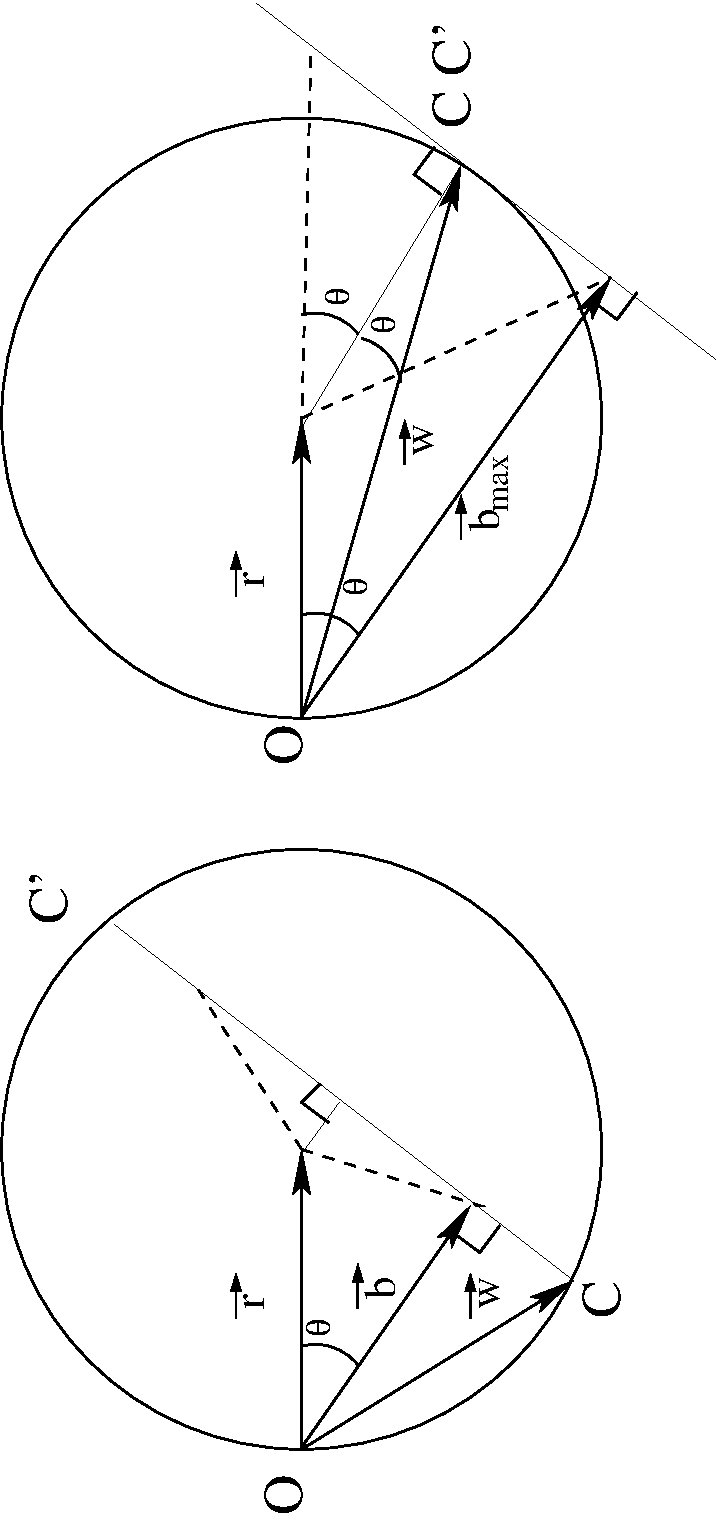
\includegraphics[angle=270,width=0.5\textwidth]{spheres.pdf}
\caption{\label{fig:spheres} Geometric construction for finding the smoothest velocity change $\vec{w}$
of the coldest atoms (with velocity $\vec{v}_C$  in the hotter region and the hottest atoms
(with velocity $\vec{v}_H$ in the colder region.  Both figures
represent a sphere of radius $\vec{r}=(\vec{v}_C -\vec{v}_H)/2$.  The plane perpendicular to {$\vec{b}$},
intersects the sphere in a circle, which is the locus of solutions $\vec{w}$ obeying energy and momentum
conservation rules.  The points $C$ and $C^\prime$ (in the $\vec{r}$--$\vec{b}$ plane) give the
solutions with least and greatest impulse.  The right-hand version shows the largest vector $\vec{b}$
which allows solutions for $\vec{w}$.  The minimum and maximum impulse solutions have
merged to a point.}
%\label{fig:spheres}
\end{figure}
\par


The energy shift criteria (i) and (ii) give equations 
$-2\vec{v}_H \cdot\vec{w} +w^2=-2\Delta/m\equiv-\delta$,
and $2\vec{v}_C \cdot\vec{w} +w^2=+\delta$.  Adding and subtracting these equations
give
%
\begin{eqnarray}
\delta&=&(\vec{v}_H + \vec{v}_C)\cdot \vec{w} \nonumber  \\
w^2 &=& (\vec{v}_H-\vec{v}_C)\cdot \vec{w},
\label{eq:geom}
\end{eqnarray}
%
a linear and a quadratic equation for $\vec{w}$.  These have a simple geometric interpretation
shown in Fig. \ref{fig:spheres}.  The first equation restricts the projection of $\vec{w}$ along 
the vector $\vec{v}_H + \vec{v}_C$.  Geometrically, this means that $\vec{w}$ lies on the plane
(shown by $C,C^\prime$ in Fig. \ref{fig:spheres})
perpendicular to the vector $\vec{b}\equiv \delta (\vec{v}_C + \vec{v}_H)/|\vec{v}_C+\vec{v}_H|^2$,
where the origin of $\vec{w}$ coincides with the origin of $\vec{b}$.
The second equation restricts $\vec{w}$ to the surface of a sphere of radius $|\vec{v}_H-\vec{v}_C|/2$,
centered at the end of the vector $\vec{r}\equiv(\vec{v}_H-\vec{v}_C)/2$, whose origin also coincides
with the origin of $\vec{w}$.  The sphere and the plane intersect on a circle, indicated by $C,C^\prime$
in Fig. \ref{fig:spheres}.   This circle is the one-dimensional family of solutions $\vec{w}$
satisfying Eqs.(\ref{eq:geom}).  It is also clear from the geometry that the shortest vector
$\vec{w}$ (the one that satisfies criterion (iii))
 is the one shown, from $O$ to $C$.  This lies in the same plane as the two known
vectors $\vec{r}$ and $\vec{b}$ (also the same plane as $\vec{v}_H$ and $\vec{v}_C$).  Therefore 
%
\begin{eqnarray}
\vec{w}&=&\alpha\vec{r} + \beta\vec{b} \nonumber \\ 
\vec{r}&=& (\vec{v}_H-\vec{v}_C)/2  \nonumber \\
\vec{b} &=& \frac{\delta(\vec{v}_H + \vec{v}_C)}{|\vec{v}_H+ \vec{v}_C|^2}.
\label{eq:defs}
\end{eqnarray}
%
These definitions allow Eqs.(\ref{eq:geom}) to be written as
%
\begin{eqnarray}
b^2&=&\vec{w}\cdot\vec{b} \nonumber  \\
w^2 &=& 2\vec{r}\cdot \vec{w}.
\label{eq:geom1}
\end{eqnarray}
%
The solution for $\vec{w}$ is
%
\begin{eqnarray}
\beta &=& 1-\alpha \frac{\vec{r}\cdot\vec{b}}{b^2} \nonumber \\
\alpha &=& 1-\sqrt{1-X}  \nonumber \\
X &=& \frac{(b^2-2\vec{b}\cdot\vec{r})b^2}{b^2 r^2 - (\vec{b}\cdot\vec{r})^2}
\label{eq:soln}
\end{eqnarray}
%
To derive this, substitute Eq.(\ref{eq:defs}) for $\vec{w}$ in terms of the
unknown coefficients $\alpha$ and $\beta$ into the Eqs.(\ref{eq:geom}).  The linear equation
is used to find $\beta$ in terms of $\alpha$.  Eliminating 
$\beta$ in favor of $\alpha$ in the quadratic equation gives a quadratic equation for
$\alpha$.  The appropriate solution is displayed in Eq.(\ref{eq:soln}).
An alternate version directly in terms of the velocities $\vec{v}_H$ and $\vec{v}_C$ is
%
\begin{equation}
%X=\frac{(4\Delta/m)^2-(8\Delta/m)(v_H^2-v_C^2)}{|\vec{v}_H-\vec{v}_c|^2 |\vec{v}_H+\vec{v}_c|^2
%-(v_H^2-v_C^2)^2}
X= (2\Delta/m) \frac{(2\Delta/m)-(v_H^2-v_C^2)}{v_H^2 v_C^2- (\vec{v}_H\cdot\vec{v}_C)^2}
\label{eq:X}
\end{equation}
%
%
\begin{equation}
\vec{w}=\frac{\alpha}{2}(\vec{v}_H-\vec{v}_C) + \left[\frac{2\Delta}{m}-\frac{\alpha}{2}(v_H^2-v_C^2)\right]
\frac{\vec{v}_H + \vec{v}_C}{|\vec{v}_H+\vec{v}_C|^2}
\label{eq:w}
\end{equation}
%
Notice that $X$ in Eq.(\ref{eq:X}) has a non-negative denominator that becomes zero in an accidental event
where $\vec{v}_H$ and $\vec{v}_C$ are parallel;  $X$ is then ill-defined,
because no solution exists.  An alternate pair of $C$ and $H$ atoms must
be chosen.  In the simulations reported in subsequent sections, we find that $\Delta$ should be chosen small,
making the numerator of $X$ in Eq.(\ref{eq:X}) negative.  Thus both $X$ and $\alpha$ are negative, contrary
to the version shown in Fig. \ref{fig:spheres}.  This does not adversely affect anything.

There is a second solution, $\alpha = 1+\sqrt{1-X} $,
corresponding to the maximum $|\vec{w}|$, designated as $C^\prime$ in Fig. \ref{fig:spheres}.
For $|\vec{b}|>b_{\rm max}$, there are no real solutions.  This corresponds to $X>1$.
The condition for the two solutions to coincide is $X=1$, which agrees with $b_{\rm max}
=r(1+\cos\theta)$, where $\theta$ is the angle between $\vec{b}$ and $\vec{r}$.  This can be 
understood from the right hand part of Fig. \ref{fig:spheres}, illustrating the case where
the circle collapses to a point.  For reasonable choices of the parameter $m\delta/2=\Delta$,
meaning values smaller than or similar to $k_B T/N_S$, solutions should always exist.

\section{Test on Lennard-Jones liquid}
\label{sec:LJL}


The LJ liquid is a simple case, used by M\"uller-Plathe \cite{FMP} to test his algorithm.
The pair potential is
%
\begin{equation}
V_{\rm LJ}=4\epsilon \left[ \left (\frac{\sigma}{r}\right)^{12} - \left (\frac{\sigma}{r}\right)^6 \right]
\label{eq:VLJ}
\end{equation}
%
The parameters for argon are $\epsilon/k_B=119.6$K
and $\sigma$ =3.405\AA.
First, we reproduce M\"uller-Plathe's results, at the same $(N,V,T)$=
2592 atoms, $\rho=N/V=0.849/\sigma^3$, and $T=0.7\epsilon/k_B=$84K. The same simulation
cell is used, of dimension $10.06 \ \times \ 10.06 \ \times 30.18 \ \sigma^3$, with
periodic boundary conditions.
The cut-off distance for the LJ potential is $3.0\sigma$.  We get the same 
answer, $\kappa$=7.1 in LJ units.

As shown in Fig. 2 of ref. \onlinecite{FMP},
and confirmed by our calculation in Fig. \ref{fig:amplitude}, 
the temperature gradient is essentially constant all the way to, and including, 
the slabs $0$ and $N_S/2=10$.  This is because thermal conductivity in a liquid is
very local.  This can be contrasted with fig. 6 of ref. \onlinecite{Zhou} or fig. 4
of ref. \onlinecite{Allen}, for crystals with non-local $\kappa$.
Gas theory is certainly not correct for a liquid; the concept of a mean-free
path is not valid.  However, we can get an idea of what happens by unlicensed use of the gas 
formula $\kappa = C{\bar v}\Lambda/3$.  The measured thermal conductivity
of liquid argon (0.132 W/mK at temperature near 100K and pressure 
near 1Mbar \cite{Younglove,argonk})
then corresponds to a mean free path $\Lambda \approx 0.14 \ \AA$, more
than 30 times smaller than the slab separation $d=1.51\sigma$.  In other words, the non-local
conductivity $\kappa(x-x^\prime)$ decays to zero by the first neighbor slab, or
$\kappa(q)$ is independent of $q$ out to values of $q$ larger than $q_{\rm max}=\pi/d$. 

\par
\begin{figure}[top]
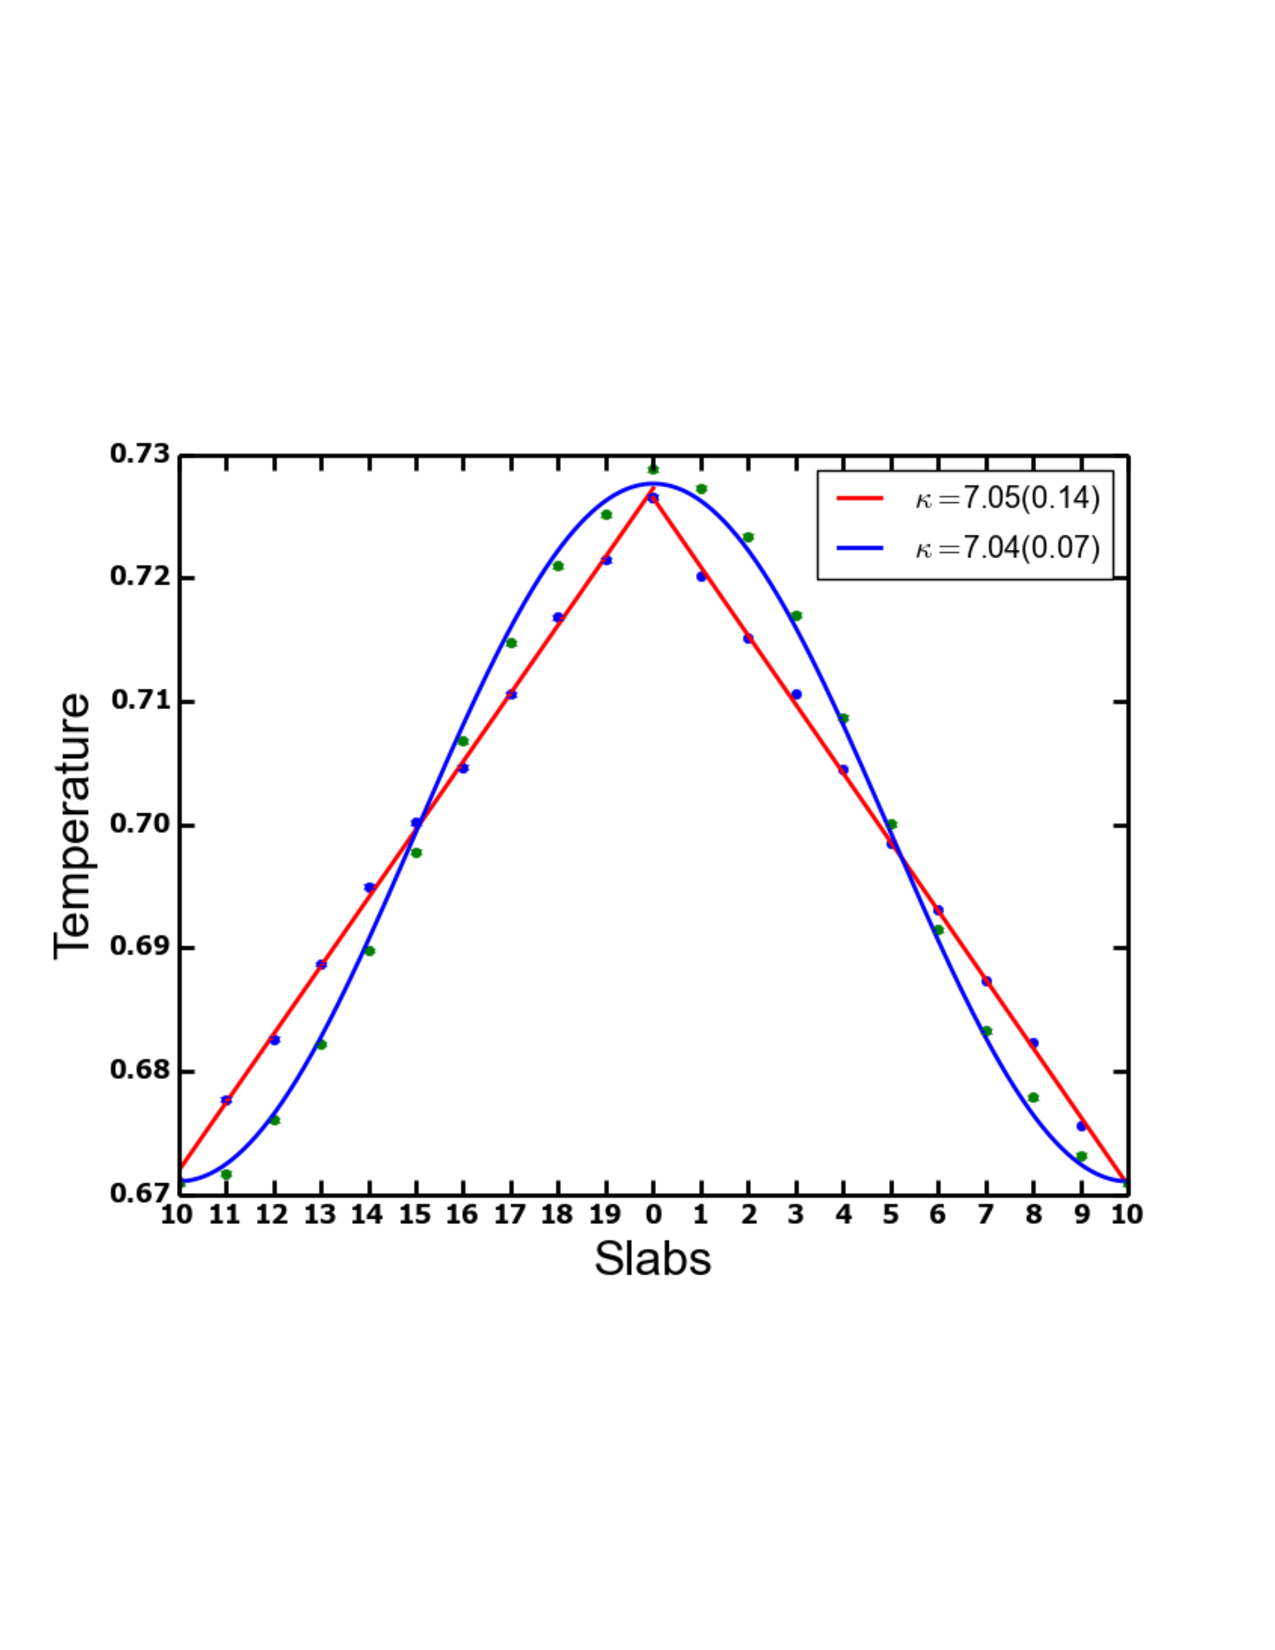
\includegraphics[angle=0,width=0.5\textwidth]{amplitude6.pdf}%{amplitude1.png}
\caption{\label{fig:amplitude} temperature profiles from direct simulations for the 
Lennard-Jones crystal.  The points fit by the straight line are a reproduction of the
calculation of M\"uller-Plathe.  The points fit by the sine curve use the same simulation
cell, and spatially sinusoidal heating and cooling.}
%\label{fig:amplitude}
\end{figure}
\par

Also shown in Fig. \ref{fig:amplitude} is the sinusoidal temperature profile gotten
numerically from our sinusoidal heating.  The computational system is unaltered.  The  
2592 atoms are in the same cell, divided into 20 slabs, at the same $T$.    Sinusoidal heat 
$N_S \dot{e}$ between 1 and 5 $\epsilon/\Delta t$ is used.  
The interval between heat injections is $\Delta t= 60\delta t$,
where the time step of the ``velocity Verlet''  Newton's-law 
integration algorithm \cite{Hansen,Verlet} is $\delta t = 0.007 t_{LJ}$.  The
Lennard-Jones unit of time for argon is $t_{LJ}=\sigma\sqrt(m/\epsilon)=2.16$ ps.
Equilibration required $10^4 \ \delta t$ of constant $T$ simulation, and $T(\ell)$ averaging was done
for $2\times10^5 \delta t$; good convergence was found in $5\times10^4 \delta t$ as shown in Fig.
\ref{fig:error}.

To estimate errors, consider that there are 130 atoms per slab, each with mean energy $k_B T$
and rms deviation of $k_B T$ from the mean, according to Maxwell-Boltzmann statistics.  
Thus the mean slab energy per atom, at any particular moment,
should be about $k_B T \pm k_B T/\sqrt 130$  Therefore, if averaged over 100 random and independent
thermalized configurations, the temperature error in a slab will be less than 1\%.  A run of
$5\times10^4 \delta t$ should be more than sufficient for this purpose.  Fig. \ref{fig:amplitude}
suggests errors of order 0.001$k_B T$ in the slab temperatures.

Compared with the M\"uller-Plathe \cite{FMP} result, both of the current ones give the same
value, $\kappa$ = 7.1 in LJ units, which is  0.133 W/mK, very close to the experimental
value for argon, 0.132 W/mK \cite{Younglove,argonk}.  The sinusoidal algorithm gives
faster convergence and a slightly more accurate final answer, as shown in
Fig \ref{fig:error}.

\par
\begin{figure}[top]
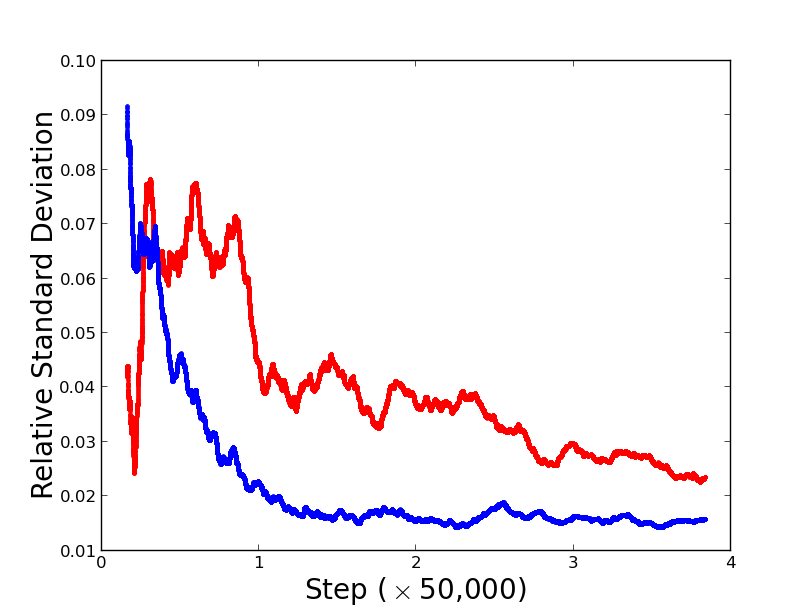
\includegraphics[angle=0,width=0.5\textwidth]{RelativeError2.png}
\caption{\label{fig:error} Time evolution of the error of simulation of $\kappa$ for the
Lennard-Jones liquid.  The upper and noisier curve uses the method of M\"uller-Plathe.
The lower curve is the result of the sinusoidal algorithm of this paper.}
\label{fig:error}
\end{figure}
\par






\section{Extrapolation}

MD answers for $\kappa$ are computed for finite size $L$.  Therefore extrapolation is required
to estimate the bulk ($L\rightarrow \infty$) answer.  Sellan {\it et al.} \cite{Sellan} have analyzed this.
It was also analyzed in the previous paper \cite{Allen}, using a Debye model.  Here we continue the analysis.
Equations (22,23) of ref. \onlinecite{Allen} are
%
\begin{equation}
\kappa(q)=\frac{1}{\Omega}\sum_Q \hbar\omega_Q\frac{\partial n_Q}{\partial T} 
v_{Qx}^2 \tau_Q \cos^2(qd/2)   F(q,\Lambda_{Qx})
\label{eq:kappaslab1}
\end{equation}
%
\begin{equation}
F(q,\Lambda)=  \left[ 1 +4\sin^2 (qd/2)
\left\{ \left( \frac{\Lambda}{d} \right) + \left( \frac{\Lambda}{d} \right)^2 \right\} \right]^{-1} ,
\label{eq:kappaslab2}
\end{equation}
%
where $v_{Qx}, \ \tau_Q$, and $\Lambda=v_{Qx}\tau_Q$ are the group velocity, quasiparticle lifetime,
and $x$-component of
mean free path of the phonon mode of frequency $\omega_Q$.   These equations solve the PBE
in relaxation-time approximation for the case where heat is applied as $\cos(q\ell d)$ with $q=2\pi/L$
and where $L$ is the periodic repeat length an infinite sample or of a model on a torus (exactly as
in the calculations of secs. \ref{sec:LJL} and \ref{sec:LJC}).  In ref. \onlinecite{Allen}, these were approximately
evaluated using a Debye model, and integrating $Q$ over a Debye sphere.  The Debye version is
%
\begin{equation}
\kappa_D(q)=\kappa_{D0} \cos^2 (qd/2) \frac{1}{N}\sum_Q \left( \frac{Q_x}{Q}\right)^2
\left(\frac{Q_D}{Q}\right)^p F(q,\Lambda_{Qx}),
\label{eq:D1}
\end{equation}
%
where $\kappa_{D0}$ is a convenient scale factor,
%
\begin{equation}
\kappa_{D0}=\frac{3N}{\Omega} k_B v^2 \tau_D,
\label{eq:D2}
\end{equation}
%
and the mean free path is
%
\begin{equation}
\Lambda_{Qx}=v\tau_D \frac{Q_x}{Q} \left(\frac{Q_D}{Q}\right)^p.
\label{eq:D3}
\end{equation}
%
The Debye wavevector has its usual value, $(6\pi^2 N/\Omega)^{1/3}$, and the exponent $p$ is
chosen to be 2.



Here, instead of integrating over the Debye sphere, we do the 
discrete sum of Eq. \ref{eq:D1} over the Brillouin zone of the {\it fcc} simulation cell
that will be used in the next section for the LJ crystal.  That is, we use only those
$\vec{Q}$'s  in the {\it fcc} Brillouin zone such that $\exp(i\vec{Q}\cdot\vec{A}_i)=1$,
where $\vec{A}_i$, for $i=1,2,3$, are the orthogonal translation vectors of the simulation
supercell.  As an example, the mesh used in Sec. \ref{sec:LJL} for the LJ liquid corresponds
to $\vec{A}_1 = 6a(1,0,0)$, $\vec{A}_2 = 6a(0,1,0)$, and $\vec{A}_3 = 18a(0,0,1)$,
where $a=1.68\sigma$ is the lattice constant of the {\it fcc} conventional cubic cell, using the
liquid argon density, 0.849/$\sigma^3$.
Our simulation cells in this and the next section will be very similar, but longer in the $\vec{A}_3$ direction,
{and with $a$ readjusted to $1.56\sigma$ to give the higher density\cite{Verlet,Ladd},
1.053/$\sigma^3$, of the low pressure LJ crystal.
The corresponding $\vec{Q}$'s are the vectors $\ell\vec{G}_1+m\vec{G}_2+n\vec{G}_3$
of the lattice reciprocal to the $\vec{A}$'s.  This
 is an anisotropic reciprocal-space mesh, being coarse in the directions $\vec{A}_1$ and $\vec{A}_2$, but finer
in the direction $\vec{A}_3$, corresponding to the actual distribution of normal modes of the atoms
in the simulation cell of the LJ crystal.  Our hypothesis is that the Debye model, with frequency
$\omega_Q = v|\vec{Q}|$ for all 3 branches, and $1/\tau_Q = (1/\tau_D)(Q/Q_D)^2$, will sufficiently
capture the physics of the LJ crystal for purposes of learning how to extrapolate to infinite
simulation cell size.  Then we will use this result to guide extrapolation of the simulations
in the next section.

First we study convergence as a function of the transverse dimension of the cell.  The
result, shown in Fig. \ref{fig:cross}, is extremely favorable, indicating that coarseness of
the $\vec{Q}$-mesh in the $\vec{A}_1$ and $\vec{A}_2$ directions is no problem.
\par
\begin{figure}[top]
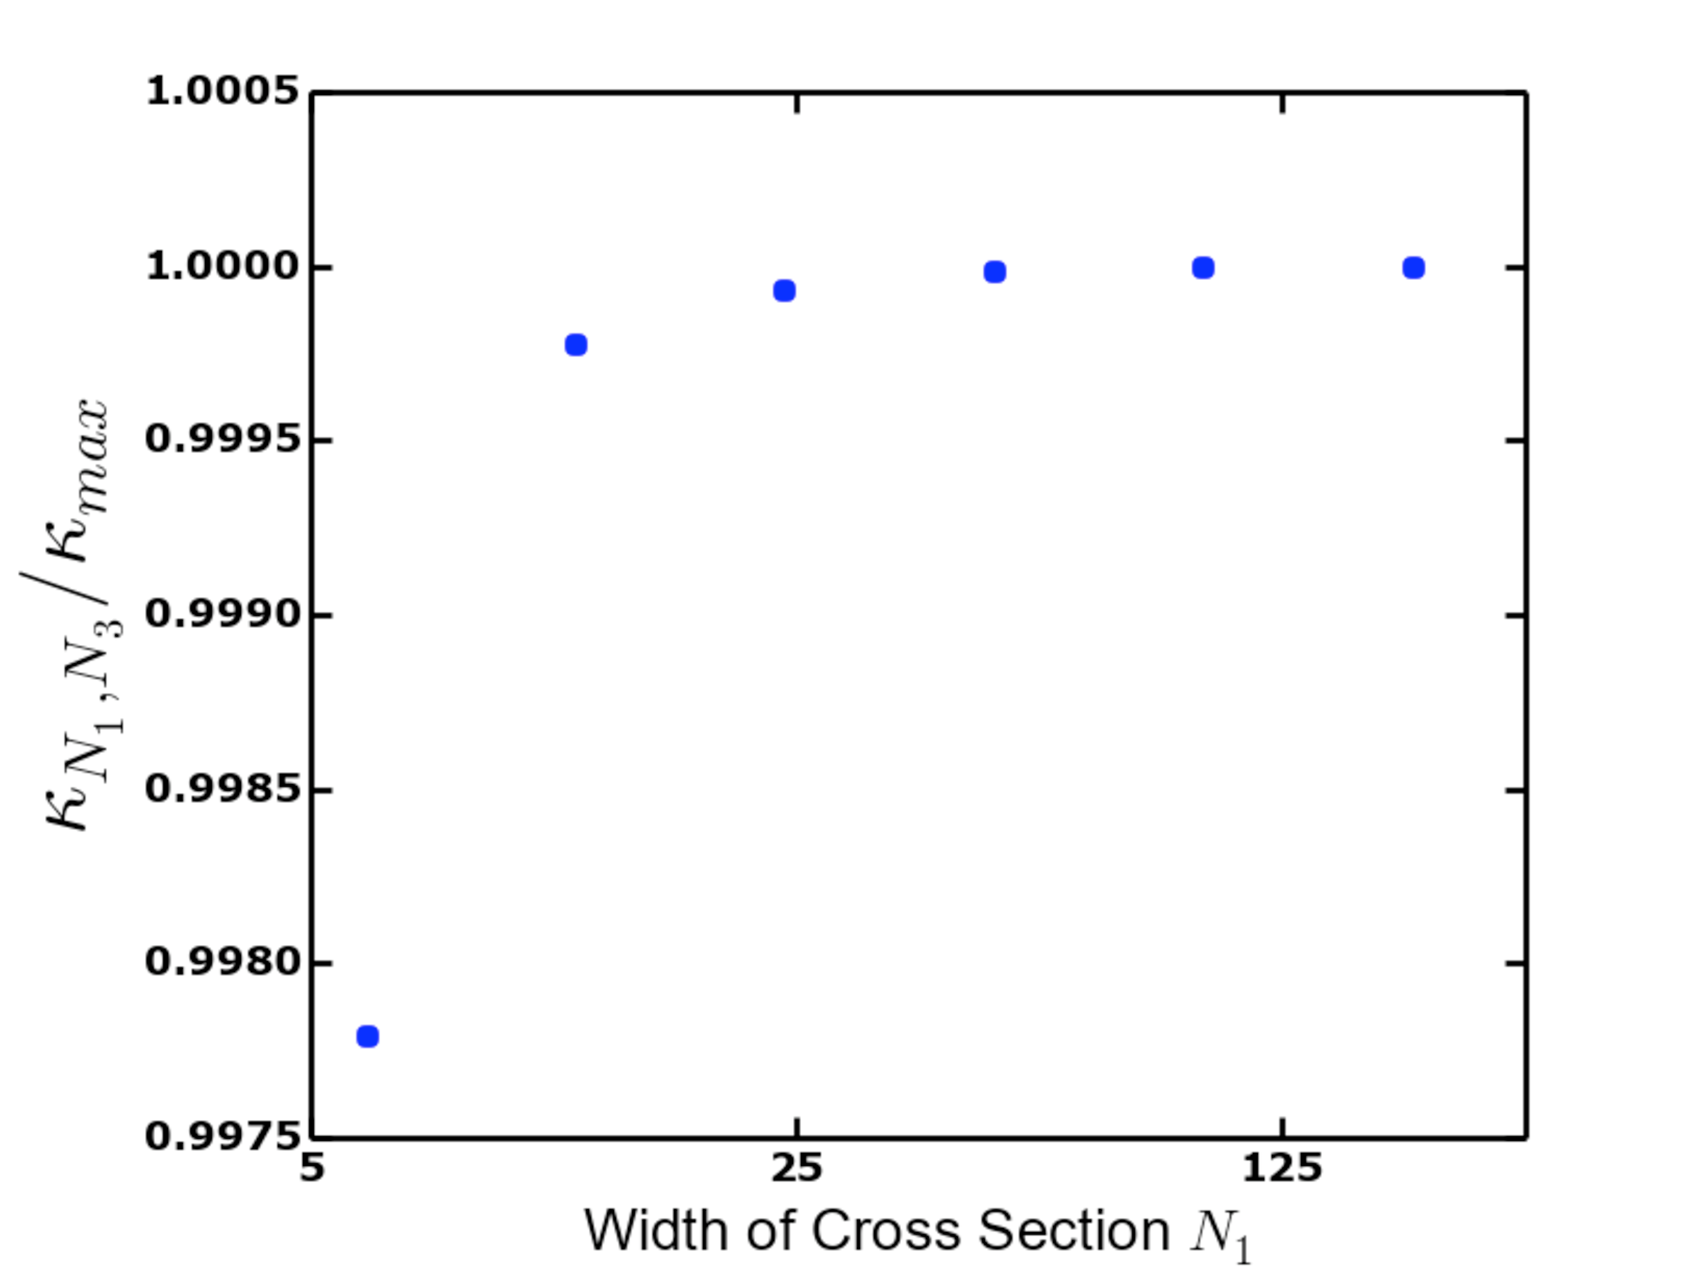
\includegraphics[angle=0,width=0.5\textwidth]{Cross14.pdf}%{Cross3.png}
\caption{\label{fig:cross} Fast convergence of $\kappa$ expected for a simulation cell
of size $N_1$, $N_1$, $N_3$, as predicted using the Debye-model version of 
Eqs.(\ref{eq:kappaslab1},\ref{eq:kappaslab2}).  The Q-sum is not over the
Debye sphere, but over the anisotropic Q-mesh corresponding to the
normal modes of the {\it fcc} crystalline LJ lattice.  The value $N_3 = 500$ was fixed,
and $\kappa_{\rm max}$ is set to the value with $N_1=192$.}
\label{fig:cross}
\end{figure}
\par

Next we study convergence as a function of the longitudinal dimension of the cell.
Here convergence is slower. {\bf Figure needed.} Fig. \ref{fig:powerlaw} is inserted
here just for temporary illustration.  The result is very similar (?) to what was found in
ref.\onlinecite{Allen} where Debye-model spherical symmetry was exploited and the mesh was isotropic.
\par
\begin{figure}[top]
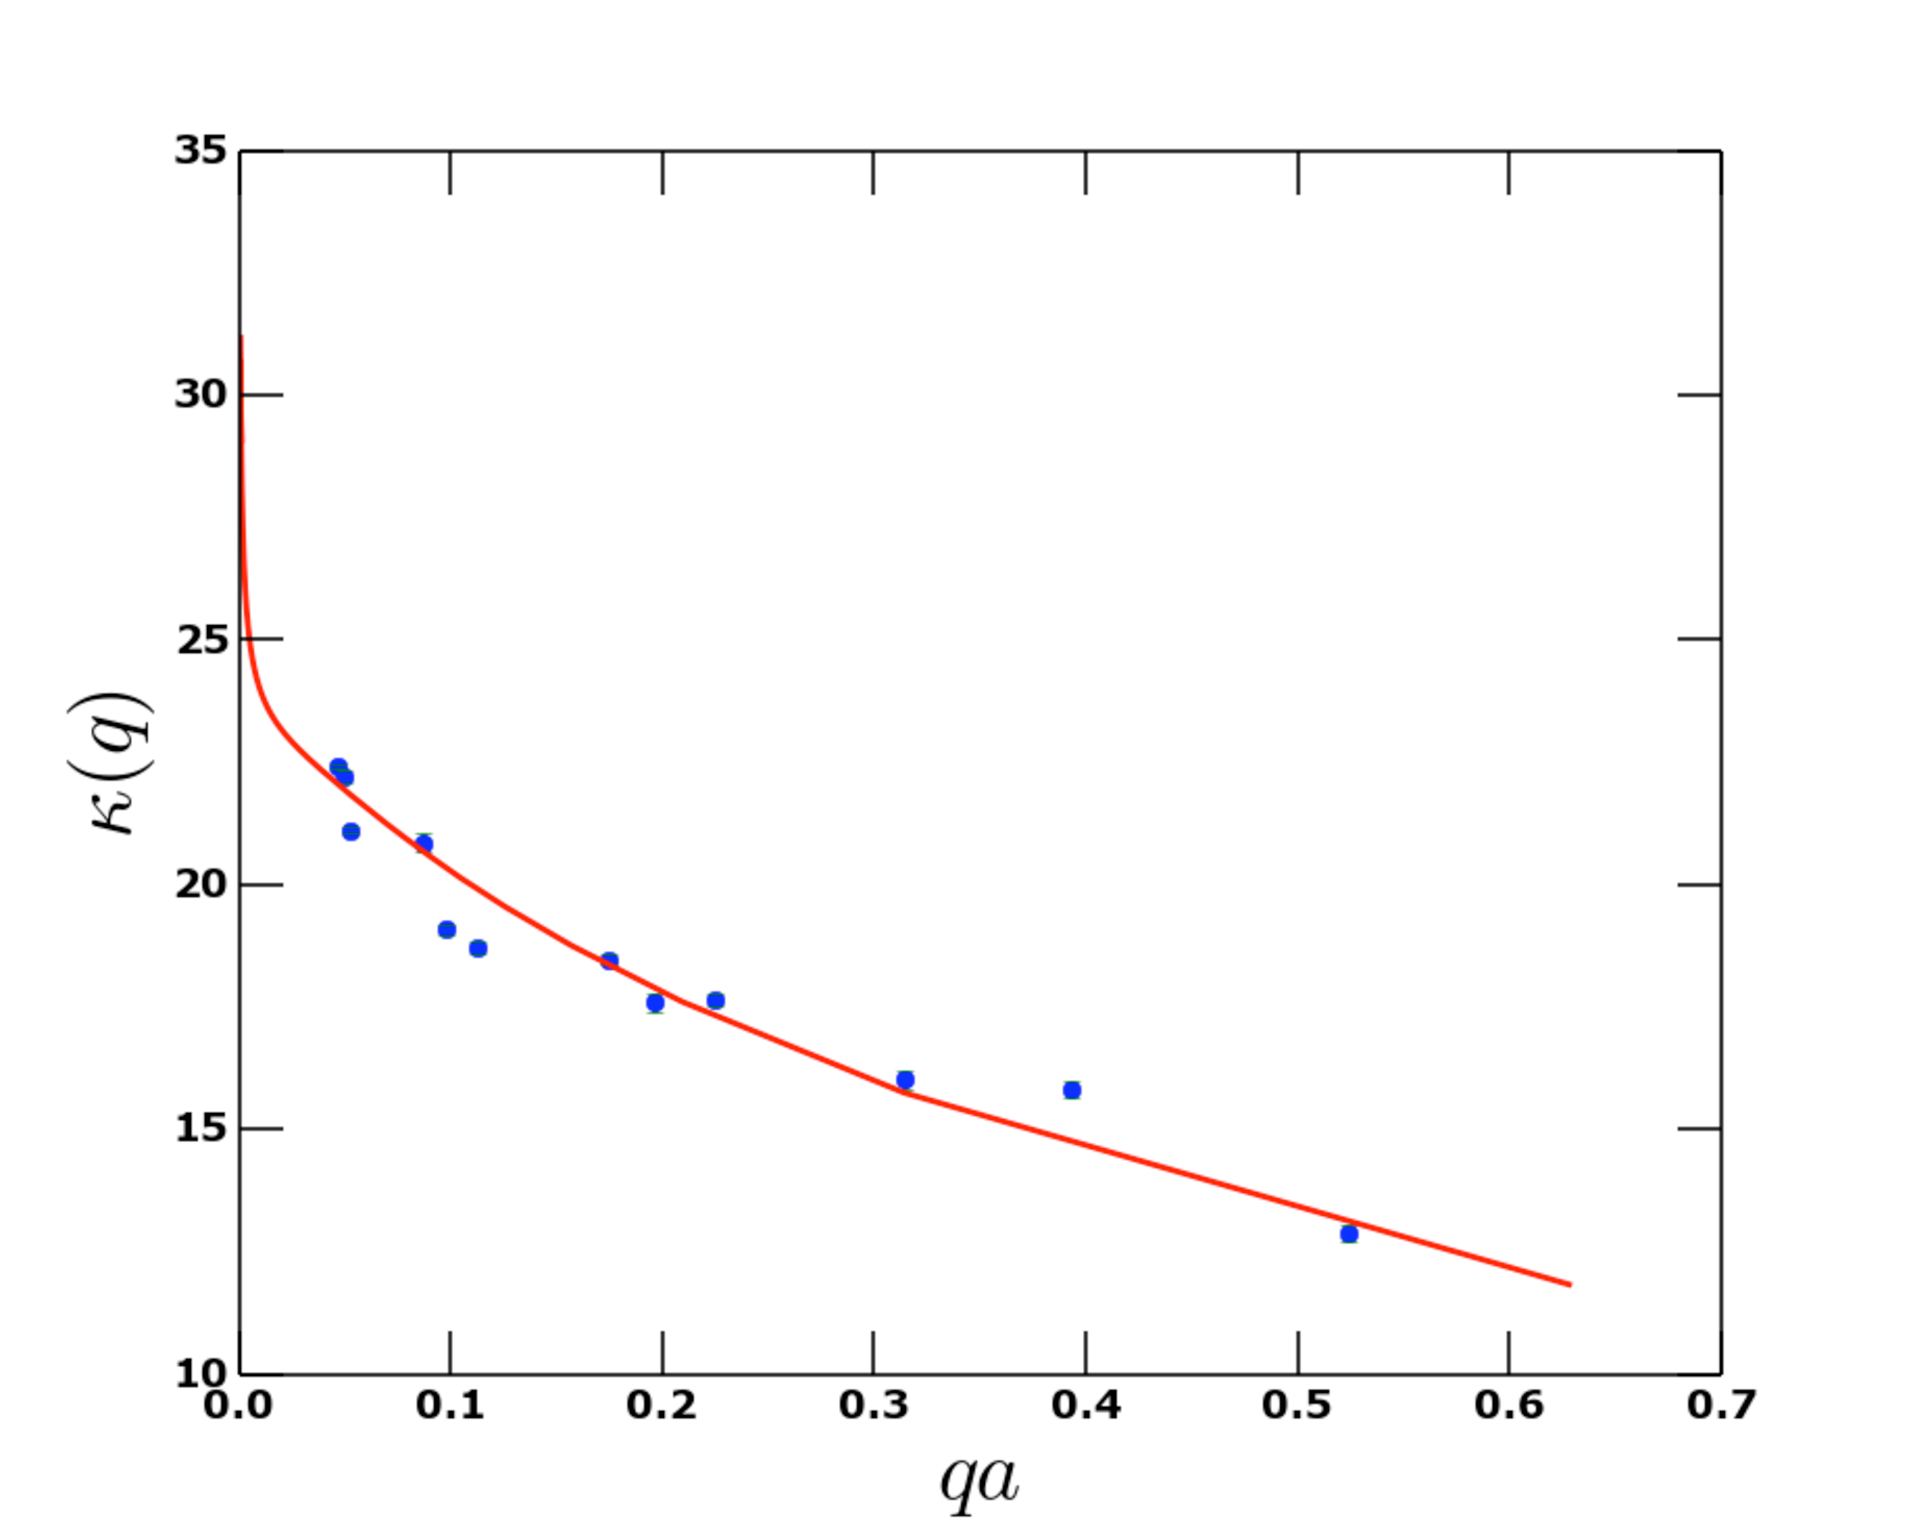
\includegraphics[angle=0,width=0.5\textwidth]{extrapolation15.pdf}%{powerlaw1.pdf}
\caption{\label{fig:powerlaw} Just an illustration.  The Debye
model is used to model expected convergence versus supercell length $L$.  The figure will
have only one curve.  It doesn't need to be this tall.  The Q-sum is not over the
Debye sphere, but over the anisotropic Q-mesh corresponding to the
normal modes of the {\it fcc} {\it fcc} LJ supercell.  The values $N_1 = N_2 = 6$ are fixed,
and $\kappa_{\rm max}$ is set to the value with $N_3=500$.}
\label{fig:powerlaw}
\end{figure}
\par


\section{Lennard-Jones crystal}
\label{sec:LJC}

For an LJ crystal, the situation is different.  Phonon gas theory
applies to fairly good approximation.   
Higher energy phonons have mean free paths
longer than the slab thickness $d$, which we choose to be $a = 5.32 \AA$.
Lower energy phonons have mean free paths $\Lambda_Q$ increasing,
roughly as $1/\omega_Q^2$.  The values of $\Lambda_Q$ are not as long as in GaN, 
modeled by Zhou {\it et al.} \cite{Zhou}.  
Doing a converged calculation by MD methods is challenging.  {\bf Need to read and
cite prior calculations.}  We use this to test whether our algorithm is helpful.   
The time step of the ``velocity Verlet''  Newton's-law 
integration algorithm \cite{Hansen,Verlet} is $\delta t = 0.007 t_{LJ}$ for shorter samples,
and $0.014 t_{LJ}$ for longer samples.

\par
\begin{figure}[top]
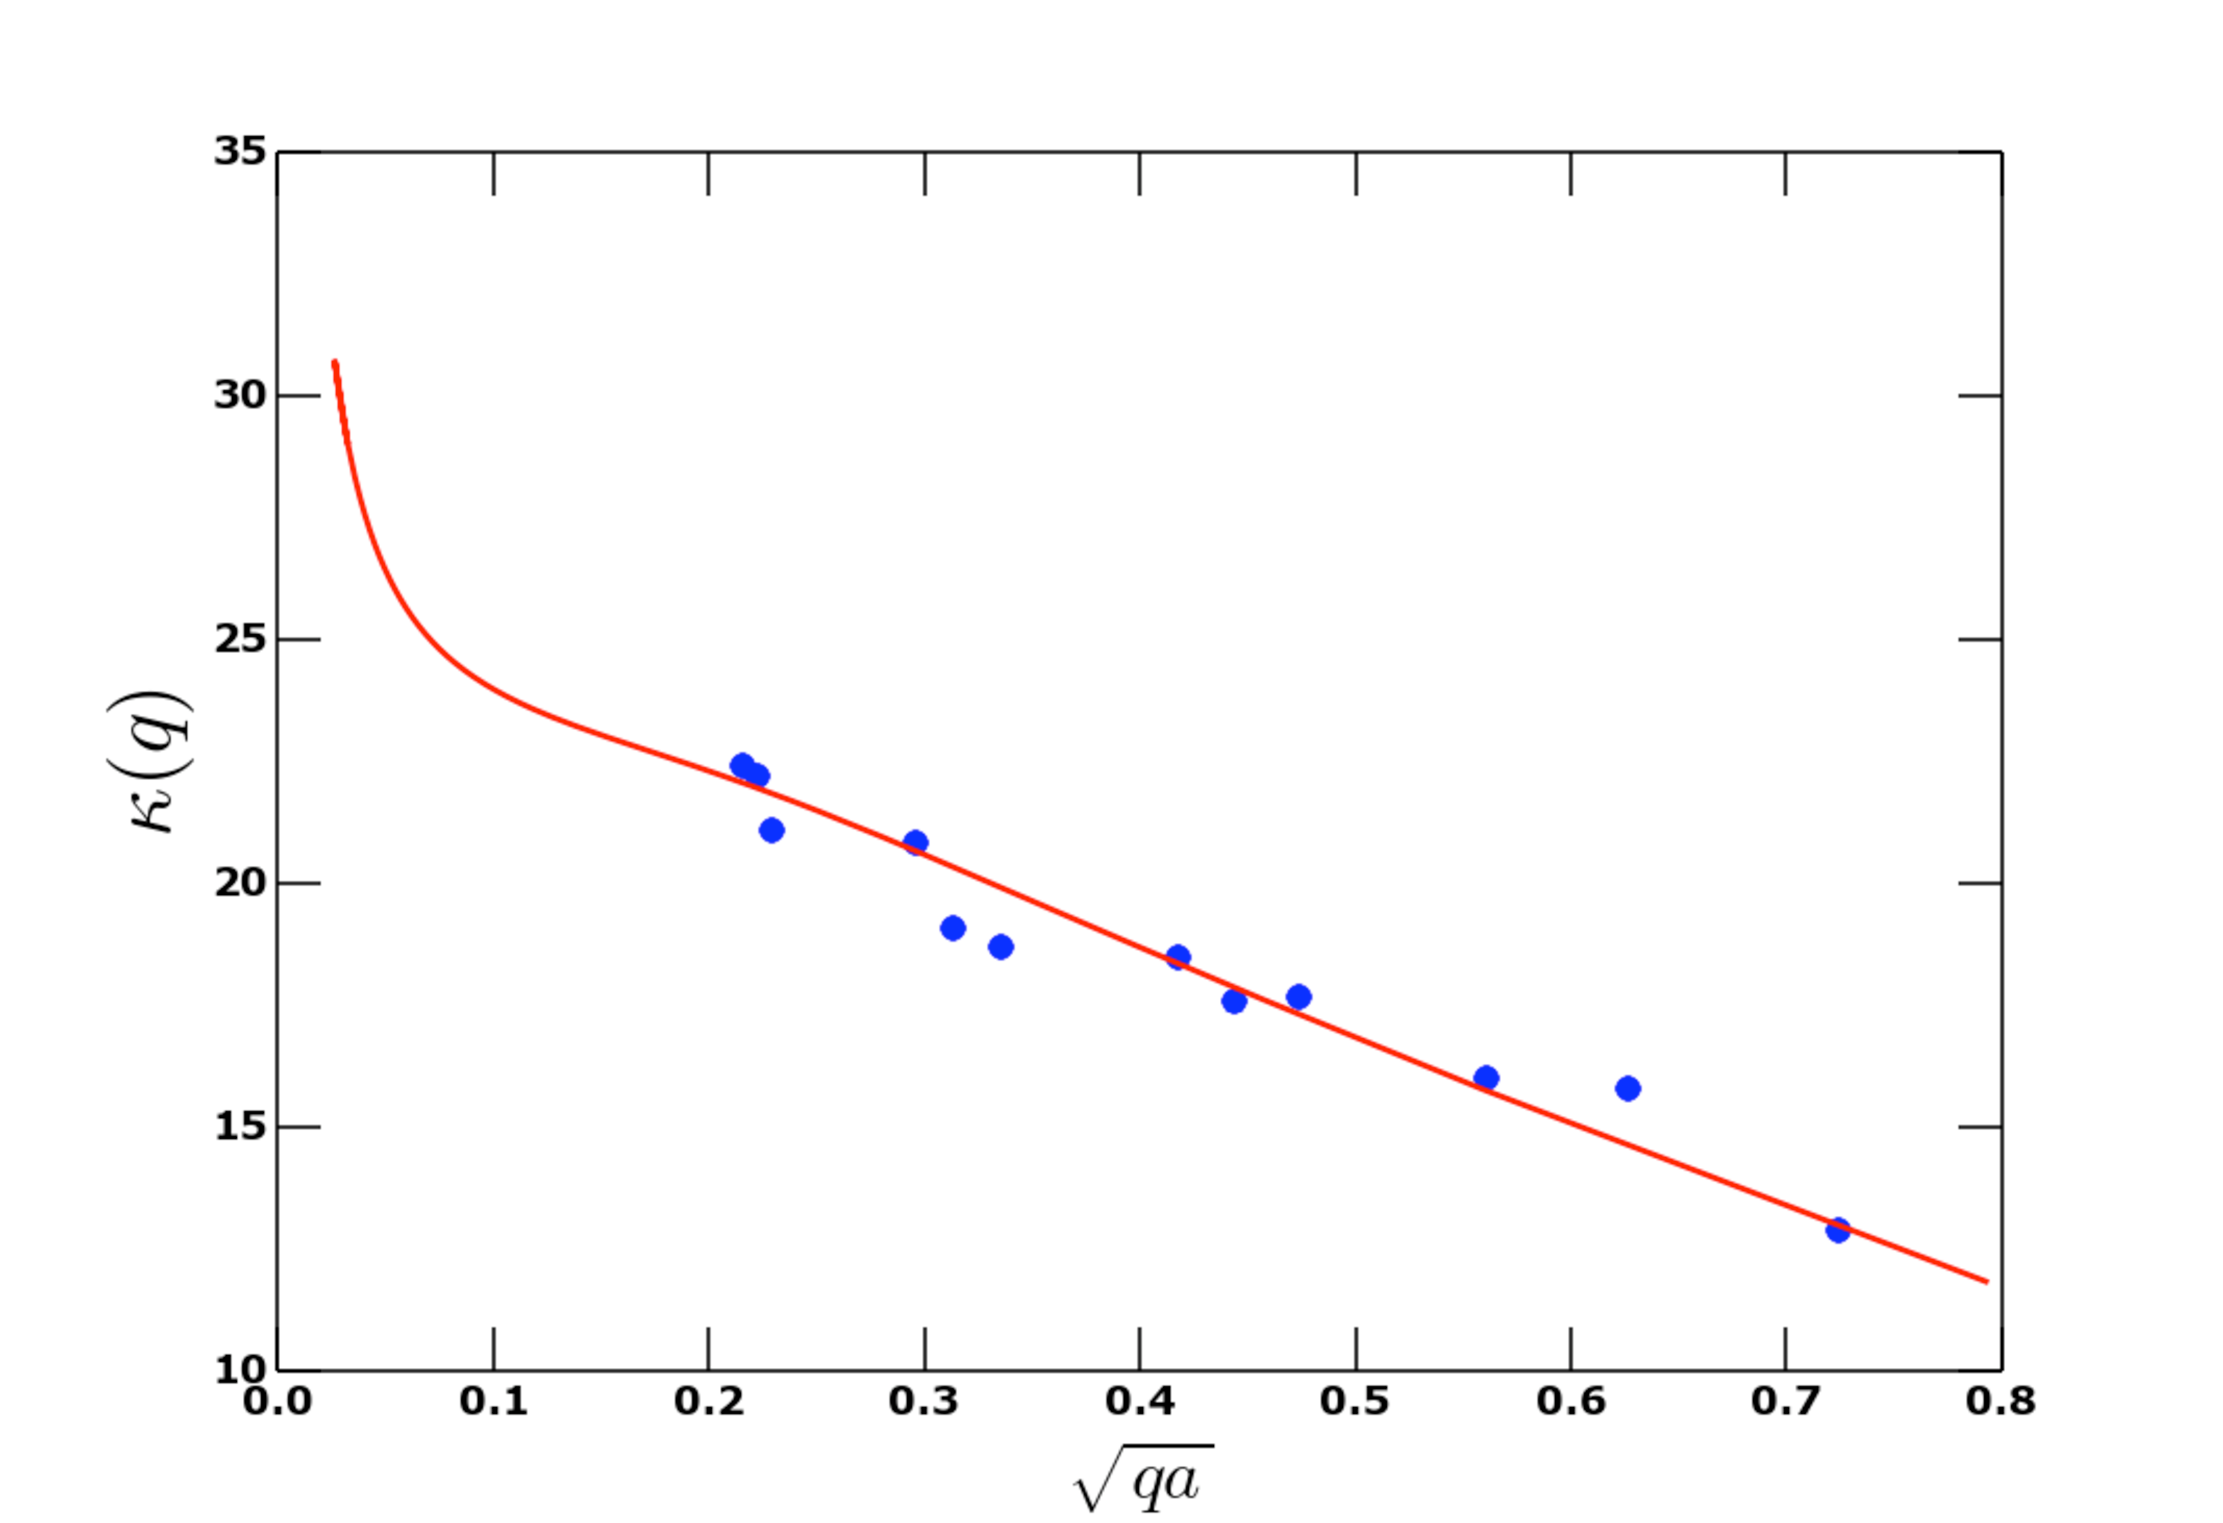
\includegraphics[angle=0,width=0.5\textwidth]{test11.pdf}%{extrapolationb3.png}
\caption{\label{fig:error1} Fourier-space $\kappa(q)$ computed numerically
at the minimum $q_{\rm min}=2\pi/L$ for various cell sizes $L$.  The values
of $\kappa$ are shown in LJ units ($\kappa_{\rm LJ}=(k_B/\sigma^2)\sqrt(\epsilon/M)$=
0.0188 W/mK). The red-line extrapolation sums over wave vectors in the first Brilloin Zone.}
\label{fig:error1}
\end{figure}
\par

At $T$ not too far above the
triple-point temperature, higher than second-order anharmonicity starts to be
noticable in LJ crystals.
This shortens the mean free paths, to the point where gas theory starts to break down.  
This has two advantages: the simulation cell does not have to be as long, and
non-Boltzmann behavior is the regime where an MD simulation is worth doing .
We have chosen to simulate crystalline LJ argon at $T$=80K, close to the experimental
triple point (84K and 0.7 atmospheres.)

Fig.\ref{fig:error1} shows results for $\kappa(q=2\pi/L)$ where $L=N_3d$ is the
length of the simulation cell, and $d=a$.  These calculations used a heat input ${\dot e}\tau$ per volume of 1.265$\epsilon$, the interval $\tau$ being $60\delta t$.

The value of $\kappa$ in argon at $T=$80 K is measured \cite{Clayton} to be in the
range 0.4 to 0.6 W/mK.  The value of
22 in LJ units obtained from Fig.\ref{fig:error1} corresponds to 0.41 W/mK.
%
%
%
\begin{appendix}
\section{Homogeneous Mesh}
%
%
Equations \ref{eq:kappaslab1} and \ref{eq:kappaslab2}, when combined, are
%
\begin{equation}
\kappa(q)=\frac{1}{\Omega}\sum_Q \hbar\omega_Q\frac{\partial n_Q}{\partial T} 
v_{Qx}^2 \tau_Q \frac{\cos^2(qd/2)}{  1 +4\sin^2 (qd/2) ( \Lambda /d )^2  }
\label{eq:A1}
\end{equation}
%
The term first order in $\Lambda/d$ is dropped because the corrections in the denominator
are only important when $\Lambda/d = v\cos\theta\tau_D(Q_D/Q)^p /d$ is large, and the
quadratic term dominates.  
In classical approximation, $ \hbar\omega_Q\frac{\partial n_Q}{\partial T} \rightarrow k_B$,
and in Debye approximation, $v_{Qx} = v\cos\theta$.  We are interested in the minimum 
wavevector $q=2\pi/L$, so $\cos(qd/2)\rightarrow 1$ and $2\sin(qd/2) \Lambda/d \rightarrow 2\pi\Lambda/L$.
Then Eq. \ref{eq:A1} becomes (for the special case $p=2$)
%
\begin{equation}
\kappa(q_{\rm min})= \frac{k_B v^2 \tau_D} {\Omega}   \sum_Q 
 \frac{ \cos^2 \theta (Q_D/Q)^2 } {  1 + \cos^2 \theta \lambda^2 (Q_D/Q)^4  }
\label{eq:A2}
\end{equation}
%
where $\lambda\equiv 2\pi v\tau_D /L=2\pi\ell_{\rm min}/L$.  In Debye approximation, for a
uniform and dense mesh ({\it i.e.} a large crystal), the sum becomes
%
\begin{equation}
\sum_Q \rightarrow \frac{3\Omega}{(2\pi)^3} 2\pi\int_0^{Q_D} dQ Q^2 \int_{-1}^1 d\cos\theta,
\label{eq:A3}
\end{equation}
%
where the factor 3 is for the three modes.  After performing the angular integral, \ref{eq:A2} becomes
%
\begin{eqnarray}
\kappa(q_{\rm min})&=& \frac{3k_B v^2 \tau_D} {2\pi^2 \lambda^2}  \int_0^{Q_D} dQ
\frac{Q^4}{Q_D^2} \nonumber \\
&\times& \left[ 1-\frac{1}{\lambda}\left( \frac{Q}{Q_D^2} \right)^2
\tan^{-1}\lambda\left( \frac{Q_D}{Q} \right)^2  \right] \nonumber \\
&=& \frac{3\kappa_{D,0}}{2\lambda^2}\int_0^1 du u^{3/2}
\left[ 1-\frac{u}{\lambda} \cot^{-1}\frac{u}{\lambda} \right].
\label{eq:A4}
\end{eqnarray}
%
Here the replacements have been made $u=(Q/Q_D)^2$ and $\tan^{-1}(1/x)=\cot^{-1}x$,
and the conductivity scale $\kappa_{D,0}=3Nk_B v^2 \tau_D/\Omega$ is used.

Next we assert the following identity, best proved by direct differentiation:
%
\begin{eqnarray}
&&h(u)=\frac{7}{2} \int du \left[ u^{3/2} - \frac{u^{5/2}}{\lambda} \cot^{-1}\frac{u}{\lambda}\right] \nonumber \\
&&=u^{5/2} + 2\lambda^2 u^{1/2} - \frac{u^{7/2}}{\lambda}\cot^{-1}\frac{u}{\lambda}
\nonumber \\
&&-\frac{\lambda^{5/2}}{\sqrt{2}}   \left[ \frac{1}{2}\log
\left( \frac{u+\sqrt{2u\lambda}+\lambda}{u-\sqrt{2u\lambda}+\lambda}\right)
+\tan^{-1}\left(\frac{\sqrt{2u\lambda}}{\lambda-u}\right) \right] \nonumber \\
\label{eq:A5}
\end{eqnarray}
%
Now we have an answer,
%
\begin{equation}
\kappa(q_{\rm min})=\frac{3}{7}\frac{\kappa_{D,0}}{\lambda^2} [h(1)-h(0)]
\label{eq:A6}
\end{equation}
%
It is necessary to be careful in evaluating $h(1)-h(0)$.  As we integrate $u$ from 0 towards 1
(as in Eq.\ref{eq:A4}), all the terms in the integral, Eq.\ref{eq:A5} have smooth behavior except
the last term, $\tan^{-1} [\sqrt(2u\lambda)/(\lambda-u)]$.  
Note that $0<\lambda<1$ since $L$ is large.   Therefore, in this term, the argument of the arctangent
increases from zero to $+\infty$, where the arctangent equals $\pi/2$, then switches to $-\infty$,
with the arctangent still equal to $\pi/2$, and finally increases toward $0$ from the negative side,
with the arctangent approaching $\pi$ from the negative side.
Therefore, the value of $\tan^{-1} [\sqrt(2u\lambda)/(\lambda-u)]$ at $u=1$ is $\pi - \tan^{-1}
[\sqrt(2\lambda)/(1-\lambda)]$.  The answer is thus
%
\begin{eqnarray}
&&\frac{7\lambda^2}{3\kappa_{D,0}}\kappa(q_{\rm min})=  
1 + 2\lambda^2  - \frac{\tan^{-1}\lambda}{\lambda} 
\nonumber \\
&&  -\frac{\lambda^{5/2}}{\sqrt{2}}   \left[ \frac{1}{2}\log
\left( \frac{1+\sqrt{2\lambda}+\lambda}{1-\sqrt{2\lambda}+\lambda}\right)
+\pi - \tan^{-1}\left(\frac{\sqrt{2\lambda}}{1-\lambda}\right) \right] \nonumber \\
\label{eq:A7}
\end{eqnarray}
%
Finally, at large sample size $L$,  the smallest mean free
path $\ell_{\rm min}=v\tau_D$ is small compared with $L$.
The parameter $\lambda$ is $2\pi\ell_{\rm min}/L$ and the leading
size-dependent correction is
%
\begin{equation}
\kappa(q_{\rm min})=\frac{5}{7}\kappa_{D,0}\left(1-\frac{3\pi}{5}\sqrt{\frac{\pi\ell_{\rm min}}{L}}\right).
\label{eq:A8}
\end{equation}
%
This result confirms the conjecture of Ref. \onlinecite{Allen} that numerical result might be best extrapolated
by plotting $\kappa$ {\it versus} $\sqrt(1/L)$.
%
%
\section{Inhomogeneous mesh}
%
%

Now our task is to reconsider how Eq. \ref{eq:A1} behaves in a finite size crystal or simulation cell,
when one dimension ($L_z\equiv L$) gets large but the other two ($L_x = L_y \equiv L_{xy}$)
remain small.  The answer is, a new non-analytic piece occurs, and rather than converging
to the $L\rightarrow \infty$ limit as $1/\sqrt{L}$ (found above for the homogeneous mesh), it
diverges as $\sqrt{L}$.  These results are specific to the power law relaxation 
$\tau_Q=\tau_D(\omega_D/\omega)^p$ with $p=2$.  The divergence is a property of a one-dimensional
wire, indicating that ballistic transport has a dominant effect in such a system.
As the width $L_x L_y$ of the wire increases, the divergent term in $\kappa(q_{\rm min})$
decreases as $a^2/L_x L_y$, restoring the better-behaved homogeneous answer.

The specific system under consideration is an fcc crystal of volume $Na^3 /4$, where
$a$ is the conventional primitive cube size, $N=4N_x N_y N_z$ is the total number of
atoms, $N_x$ and $N_y$ being small integers held fixed, and $N_z$ being a large
integer.  We seek the behavior as $N_z$ gets very large.
The conductivity is given by Eq. \ref{eq:A2}, rewritten as 
%
\begin{equation}
\frac{\kappa(q_{\rm min})}{\kappa_{D,0}}=\frac{1}{N} \sum_{Q_z} \sum_{Q_x,Q_y} 
 \frac{ (Q_z/Q)^2 (Q_D/Q)^2 } {  1 +(Q_z/Q)^2  \lambda^2 (Q_D/Q)^4  },
\label{eq:B1}
\end{equation}
%
where $\lambda=2\pi\ell_{\rm min}/L$, $\ell_{\rm min}$ being the mean free path of the 
highest frequency phonons.
The $Q$-vectors are $\vec{Q}=(2\pi/a)(n_x/N_x,n_y/N_y,n_z/N_z)$.  This choice is required
to make vibrational normal modes satisfy periodicity in the supercell.  There are
$N$ $Q$-vectors in the Brillouin zone.
The Debye model simplifies summation over the Brillouin zone by using the Debye
sphere, with a volume equal to $n$ time the volume of the primitive Brillouin zone, $n$
being the number of atoms in the primitive cell, 4 for fcc.  The $Q$-points are
dense along the $z$ direction and sparse in the others.  Only the $Q_z$-sum
can be turned into an integral.  It is consistent with the philosophy of the Debye
model, to not use a sphere in this case, but a cube-shaped Brillouin zone, of 
volume $n$ times $(2\pi/a)^3$.  The $Q_z$ sum is then an integral, going from the smallest
non-zero $Q_z$, $2\pi/L$, ending at the largest, $Q_D=n^{1/3}\pi/a$, and multiplied by 2
to cover both negative and positive $Q_z$.  
%
\begin{equation}
\frac{\kappa(q_{\rm min})}{\kappa_{D,0}}=\frac{1}{N_x N_y} 
\sum_{Q_x,Q_y} \frac{a}{\pi}\int_{2\pi/L}^{Q_D} dQ
 \frac{ (Q_z/Q)^2 (Q_D/Q)^2 } {  1 +(Q_z/Q)^2  \lambda^2 (Q_D/Q)^4  }
\label{eq:B2}
\end{equation}
%

The number of terms in the $Q_x,Q_y$ sum is $\approx n^{2/3}N_x N_y$, typically 50
for an MD simulation, or a few thousand for a small nanowire.  Of these terms, the one
which requires special attention is the $Q_x = Q_y = 0$ term.  We denote this
term by $\kappa_{00}(q_{\rm min})$,
%
\begin{eqnarray}
\frac{\kappa_{00}(q_{\rm min})}{\kappa_{D,0}}&=&\frac{1}{N_x N_y} 
\frac{a}{\pi}\int_{2\pi/L}^{Q_D} dQ \frac{Q^2 Q_D^2 } {  Q^4 + \lambda^2 Q_D^4  }\nonumber \\
&=& \frac{n^{1/3}}{2N_x N_y}\int_\epsilon^1 dx \frac{x^2}{x^4 + \lambda^2},
\label{eq:B3}
\end{eqnarray}
%
where the variable $x$ is $Q/Q_D$ and $\epsilon=2a/n^{1/3}L$.
The integral diverges as $\lambda\rightarrow 0$.  Using very similar algebra to that
of Appendix A, the answer is
%
\begin{equation}
\frac{\kappa_{00}(q_{\rm min})}{\kappa_{D,0}}= \frac{n^{1/3}}{2N_x N_y}
\left[\frac{\pi}{2}\sqrt{\frac{L}{4\pi\ell_{\rm min}}} - 1 + \ {\rm terms \ of \ order} \ \frac{1}{L}\right]
\label{eq:B4}
\end{equation}
%

The Debye model is reliable as a guide for the low frequency behavior, provided the
relaxation-time approximation and the associated power law $p$ are correct.  The
conclusion is a bit surprising.  It indicates that if anisotropic simulation cells are used
for ``direct'' MD simulation of $\kappa$, then the extrapolation to very long cells suffers
from an unintended 1D singularity.  The product $N_x N_y$ should increase approximately
as rapidly as $N_z^{1/2}$ to prevent this term distorting the extrapolated answer.
In actual simulations, this is probably more a sobering thought than a serious warning.
But the effect is real, and shows up in the Debye-model numerics shown in Figs. 
\ref{fig:powerlaw} and \ref{fig:error1}. 




\end{appendix}



\section{acknowledgements}
We thank A. J. H. McGaughey for helpful advice.
We thank the Stony Brook University Institute for Advanced Computational Science (IACS) 
for time on their computer cluster.
This work was supported in part by DOE grant No. DE-FG02-08ER46550.

\begin{thebibliography}{99}
\bibitem{Visscher} D. N. Payton, M. Rich, and W. M. Visscher, Phys. Rev. {\bf 160}, 706 (1967).
\bibitem{Schelling} P. K. Schelling, S. R. Phillpot, and P. Keblinsky, Phys. Rev. B {\bf 65}, 144306 (2002).
\bibitem{Allen} P. B. Allen, Phys. Rev. B {\bf 90}, 054301 (2014).
\bibitem{Mahan} G. D. Mahan and F. Claro, Phys. Rev. B {\bf 38}, 1963 (1988).
\bibitem{Liang} Z. Liang and P. Keblinski, Phys. Rev. B {\bf 90}, 075411 (2014).
\bibitem{Kapres} D. G. Cahill {\it et al.}, Appl. Phys. Rev. {\bf 1}, 011305 (2014).
\bibitem{AllenFeldman} P. B. Allen and J. L. Feldman, Phys. Rev. B {\bf 48}, 12581 (1993).
\bibitem{FMP} F. M\"uller-Plathe, J. Chem. Phys. {\bf 106}, 6082 (1997).
\bibitem{Cao} B.-Y. Cao and Y.-W. Li, J. Chem. Phys. {\bf 133}, 024106 (2010).
\bibitem{Zhou} X. W. Zhou, S. Aubry, R. E. Jones, A. Greenstein, and P. K. Schelling,
Phys. Rev. B {\bf 79}, 115201 (2009).
\bibitem{Younglove}  B. A. Younglove and H. J. M. Hanley . Phys. Chem. Ref. Data {\bf 15}, 1323 (1986); 
G. A. Cook, {\it Argon, Helium and the Rare Gases}, Intersciences: NY, 1961.
\bibitem{argonk} H. J. M. Hanley, R. D. McCarthy, and W. M. Hayes, J. Phys. Chem. Ref. Data
{\bf 3}, 979 (1974); H. Ziebland and T. Burton, Brit. J. Appl. Phys. {\bf 9}, 52 (1958).
\bibitem{Hansen} J. P. Hansen and L. Verlet, Phys. Rev. {\bf 184}, 151 (1969).
\bibitem{Verlet} M. E. Tuckerman, B. J. Berne, and G. J. Martyna, J. Chem. Phys. {\bf 94}, 6811 (1991).
%\bibitem{Lee} S. H. Lee, D. K. Park, and D. B. Kang, Bull. Korean Chem. Soc. {\bf 24}, 178 (2003).
\bibitem{Sellan} D. P. Sellan, E. S. Landry, J. E. Turney, A. J. H. McGaughey, and C. H. Amon,
Phys. Rev. B {\bf 81}, 214305 (2010).
\bibitem{Ladd} A. J. C. Ladd and L. V. Woodcock, Mol. Phys. {\bf 36}, 611 (1978).
\bibitem{Clayton} F. Clayton and D. N. Batchelder, J. Phys. C {\bf 6}, 1213 (1973).
%\bibitem{Hardy} R. J. Hardy, Phys. Rev. {\bf 132}, 168 (1963).
%\bibitem{Tolman} R. C. Tolman and P. C. Fine, Rev. Mod. Phys. {\bf 20}, 51 (1948).
%\bibitem{Dames} C. Dames and G. Chen, Thermal Conductivity of Nanostructured
%Thermoelectric Materials, CRC Handbook, edited by M. Rowe
%(Taylor and Francis, Boca Raton, FL, 2006), Ch. 42.
%\bibitem{Chen} G. Chen, {\it Nanoscale energy Transport and Conversion}, Oxford University Press, 2005, Ch. 7.
%\bibitem{Zhang} Z. M. Zhang, {\it Nano/Microscale Heat Transfer}, McGraw-Hill, New York, 2007, Ch. 5.
%\bibitem{Cahill} D. G. Cahill, W. K. Ford, K. E. Goodson, G. D. Mahan, A. Majumdar, H. J. Maris, R. Merlin, and S. R. Phillpot,
%J. Appl. Phys. {\bf 93}, 793 (2003).
%\bibitem{Peierls} R. Peierls, Ann. Phys. {\bf 3}, 1055 (1929).
%\bibitem{Ziman} J. M. Ziman, {\it Electrons and Phonons}, Oxford University Press, 1960.
%\bibitem{Herring} C. Herring, Phys. Rev.%
%\bibitem{Broido} D. Broido
%\bibitem{Landauer} R. Landauer, Z. Phys. B - Condensed Matter {\bf 68}, 217 (1987).
%\bibitem{Meir} Y. Meir and N. S. Wingreen, Phys. Rev. Lett. {\bf 68}, 2512 (1992).
%\bibitem{thermostat} P. H\"unenberger, Adv. Polym. Sci. {\bf 173}, 105 (2005).
%\bibitem{Debye} P. Debye, {\it Equation of state and quantum hypothesis, with an appendix
%on thermal conductivity} (German text), in {\it Lectures on the Kinetic
%Theory of Matter and Electricity}, M. Planck, {\it et al.}, editors,
%Leipzig, Teubner, 1914, p. 19-60.
%\bibitem{Sun} T. Sun and P. B. Allen, Phys. Rev. B {\bf 82}, 224305 (2010).
%\bibitem{Krumhansl} C. Horie and J. A. Krumhansl, Phys. Rev. {\bf 136}, A1397 (1964).
%\bibitem{Pauli} W. Pauli, 1928 {\it Sommerfeld Festschrift}, Leipzig, 1928.
%\bibitem{Landau} L. D. Landau and E. M. Lifshitz, {\it Statistical Physics, 3rd Edition, Part 1}, Pergamon, Oxford, 1980, p. 160.




\end{thebibliography}

%\end{spacing}
\end{document}